\chapter{Design}
\label{cap:design}

\intro{In questo capitolo viene descritta la struttura dell'applicazione seguendo un approccio top-down, partendo quindi dal frontend per poi passare al backend descrivendo \glox{API} e database.}

\section{Premessa}

Nonostante lo stage si basasse sul lavorare ad un'applicazione già esistente, è stato comunque necessario realizzare uno studio riguardo la struttura di tale app, cercando di individuarne architettura e pattern utilizzati. L'oggetto di questo capitolo, pertanto, non sarà la descrizione di un'architettura realizzata durante lo stage, bensì la descrizione dell'architettura già presente nell'applicazione, alla quale mi sono dovuto adattare per effettuare le modifiche e aggiunte necessarie al progetto.\\
Ho ritenuto quindi l'approccio \emph{top-down} il più ragionevole da adottare, in quanto rispecchia la metodologia di studio da me seguita.

\section{Panoramica}

L'applicazione ha un'architettura a microservizi, come illustrato nella \figref{fig:microservizi}. Il suo funzionamento si basa su tre database (CommonDb, SysDb e il database aziendale contenente i dati da utilizzare) e due tipologie di \glox{API} (gateway e data provider).\\
Per utilizzare l'applicazione è necessario effettuare una login. Questa utilizza le \glox{API} gateway che interrogano il CommonDb, in particolare la tabella Utente, che contiene username e password di tutti gli utenti dell'applicazione.\\
Dopo aver effettuato la login è possibile utilizzare l'app, e ogni volta che dei dati vengono caricati dal o nel database aziendale viene messa in atto la seguente procedura:
\begin{enumerate}
    \item l'applicazione fa una chiamata alle \glox{API} gateway;
    \item queste ricavano dal CommonDb l'url delle \glox{API} data provider dell'azienda associata all'utente registrato;
    \item viene effettuata una chiamata alle \glox{API} dell'azienda (\glox{API} data provider), le quali interrogano il SysDb, per ricavare i parametri di connessione al database aziendale.
\end{enumerate}
I dettagli dell'architettura di ogni parte dell'applicazione verranno illustrati nelle sezioni seguenti.

\begin{figure}[H]
    \centering 
    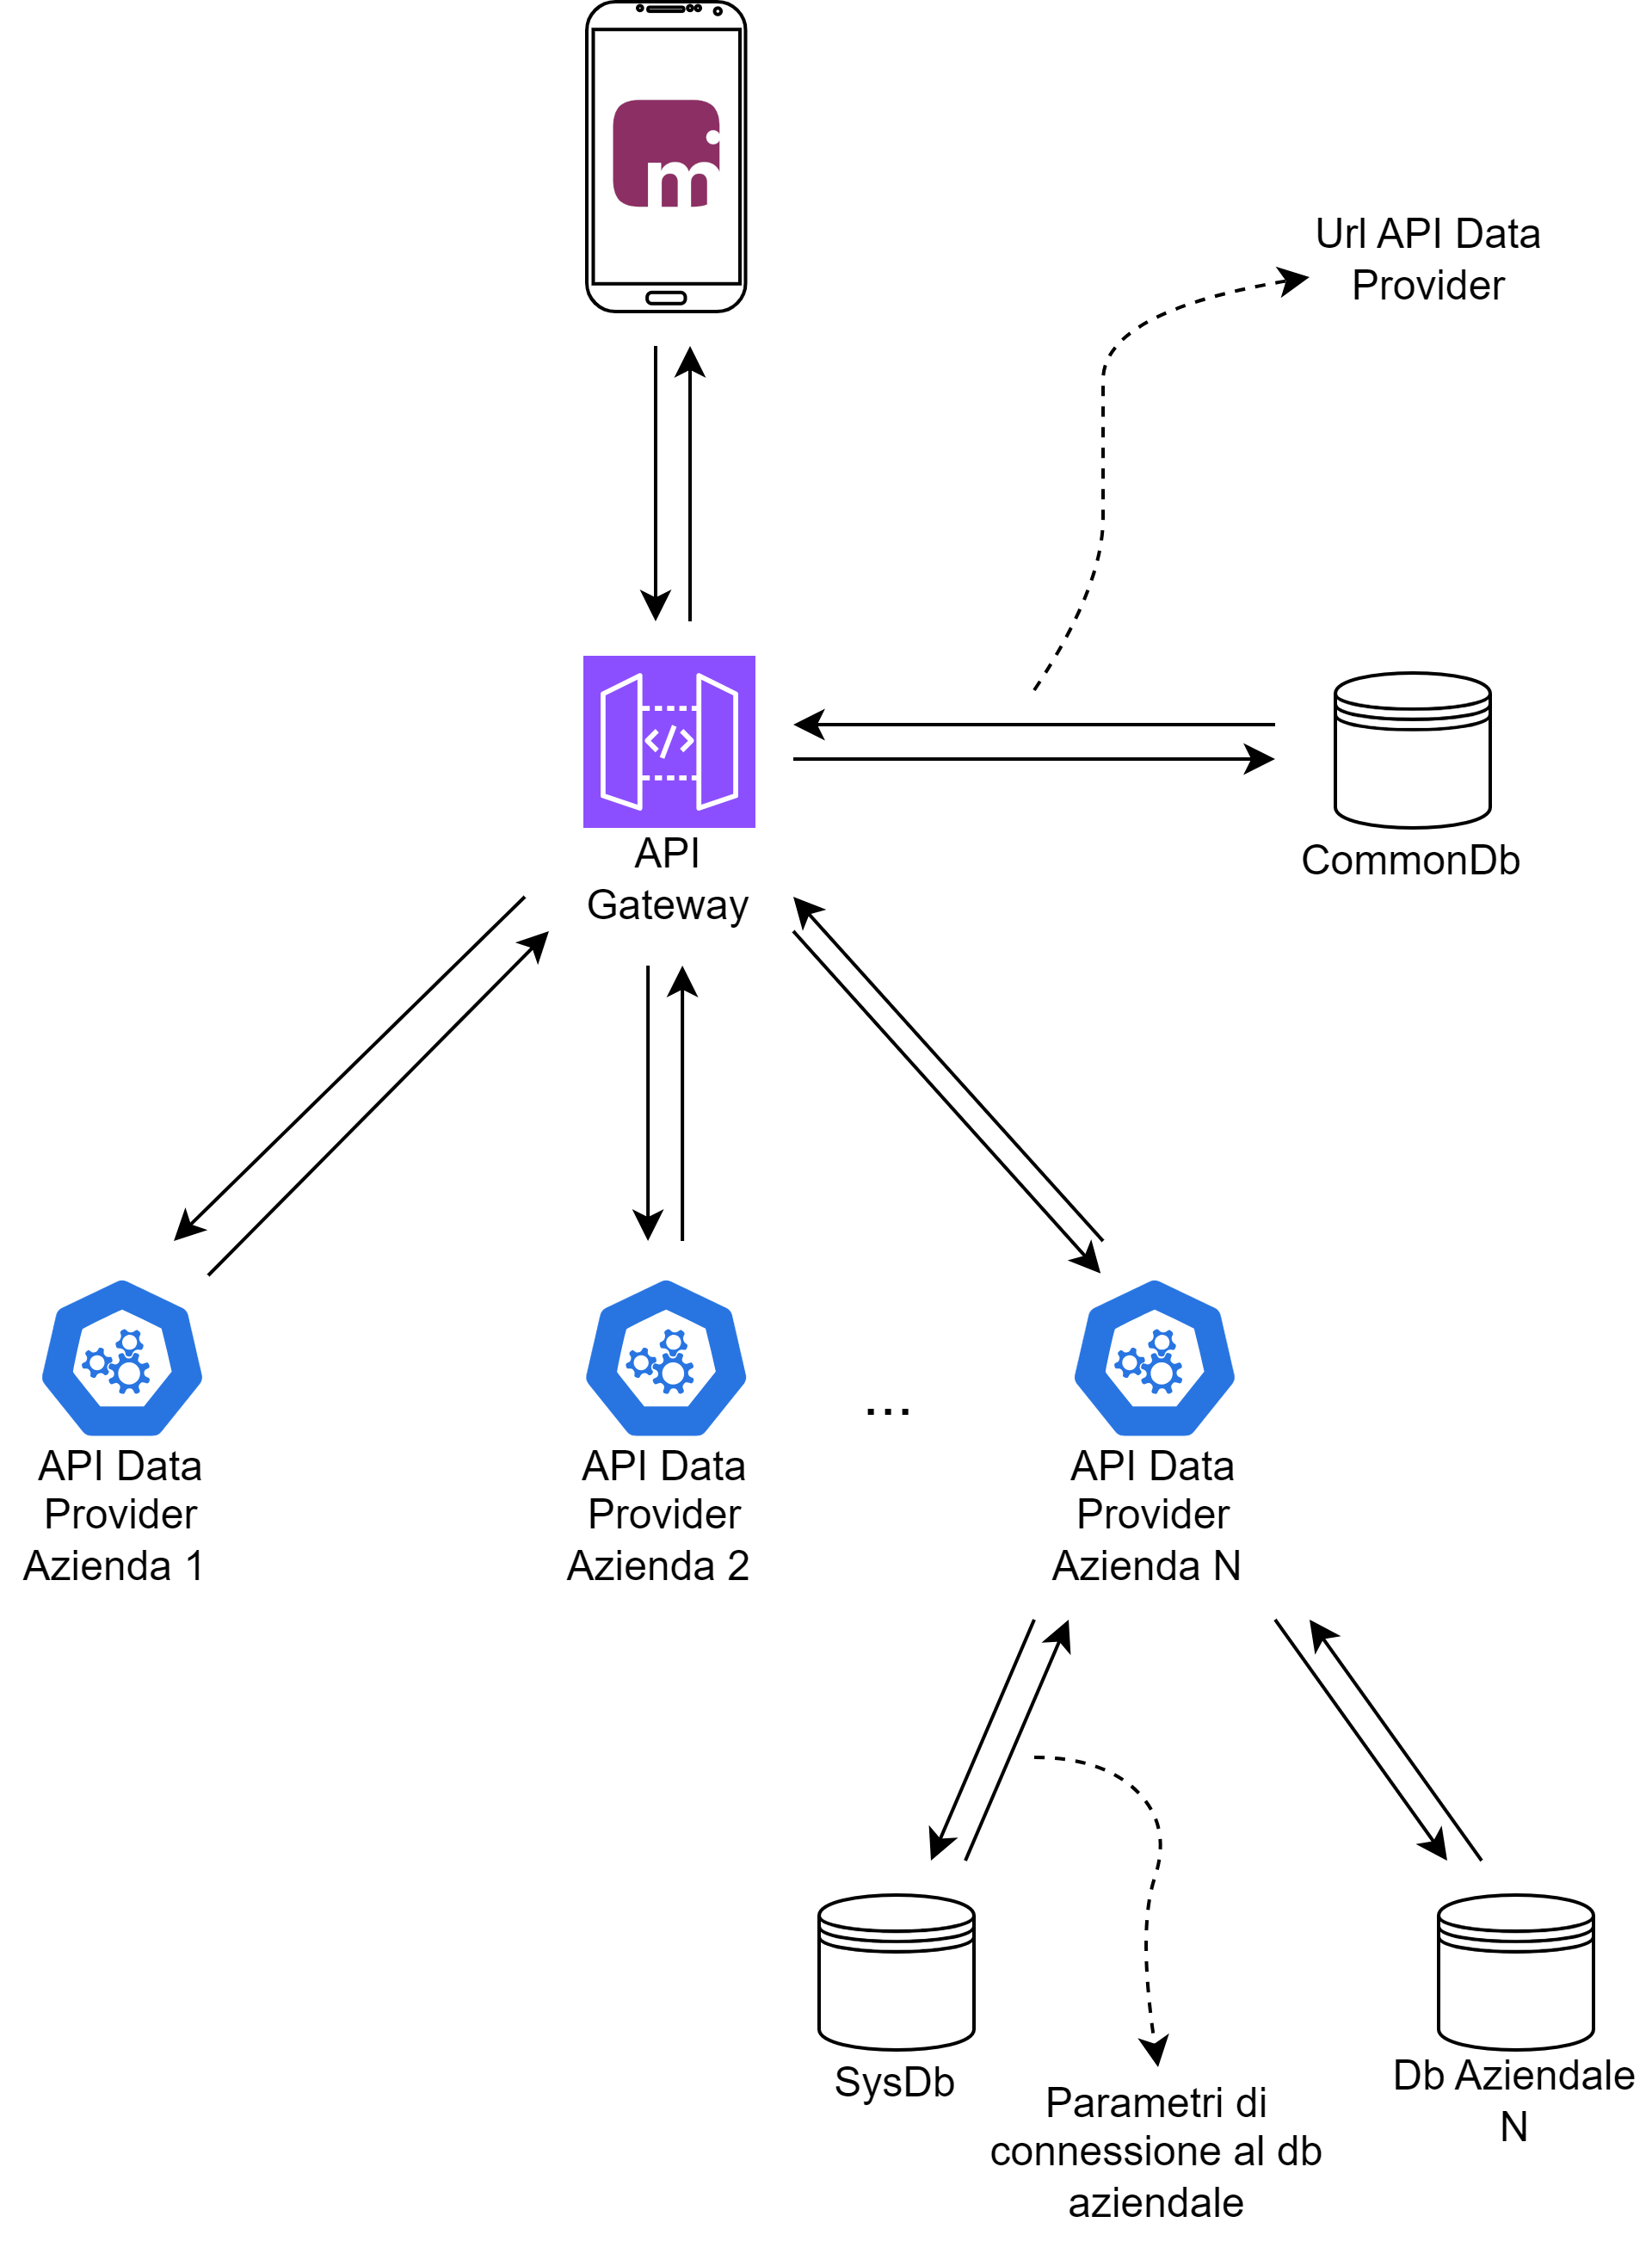
\includegraphics[width=.8\columnwidth]{images/architettura moviEXPENSE.png} 
    \caption{Architettura di moviEXPENSE}
    \label{fig:microservizi}
\end{figure}

\section{Frontend}

Il frontend di moviEXPENSE è stato realizzato con il framework Xamarin, il quale impone l'utilizzo del pattern architetturale \emph{Model-View-ViewModel} (MVVM). Questo pattern è molto utile per separare la logica dell'applicazione dall'interfaccia grafica, rendendo l'applicazione più semplice da modificare e testare. MVVM, infatti, separa il frontend in tre parti:
\begin{itemize}
    \item \textbf{Model}: contiene tutte le classi dei dati di modello, ovvero tutti i dati strutturati che appartengono al dominio dell'applicazione;
    \item \textbf{View}: si occupa della rappresentazione grafica delle informazioni. Rappresenta dunque l'interfaccia utente, occupandosi della sua struttura e della sua presentazione;
    \item \textbf{ViewModel}: implementa le proprietà e i comandi con cui la View può effettuare dei \emph{data binding}. Presenta anche un sistema di notifiche verso la View che permette di segnalare ogni cambiamento che avviene ai dati durante l'esecuzione del programma.
\end{itemize}

\begin{figure}[H]
    \centering 
    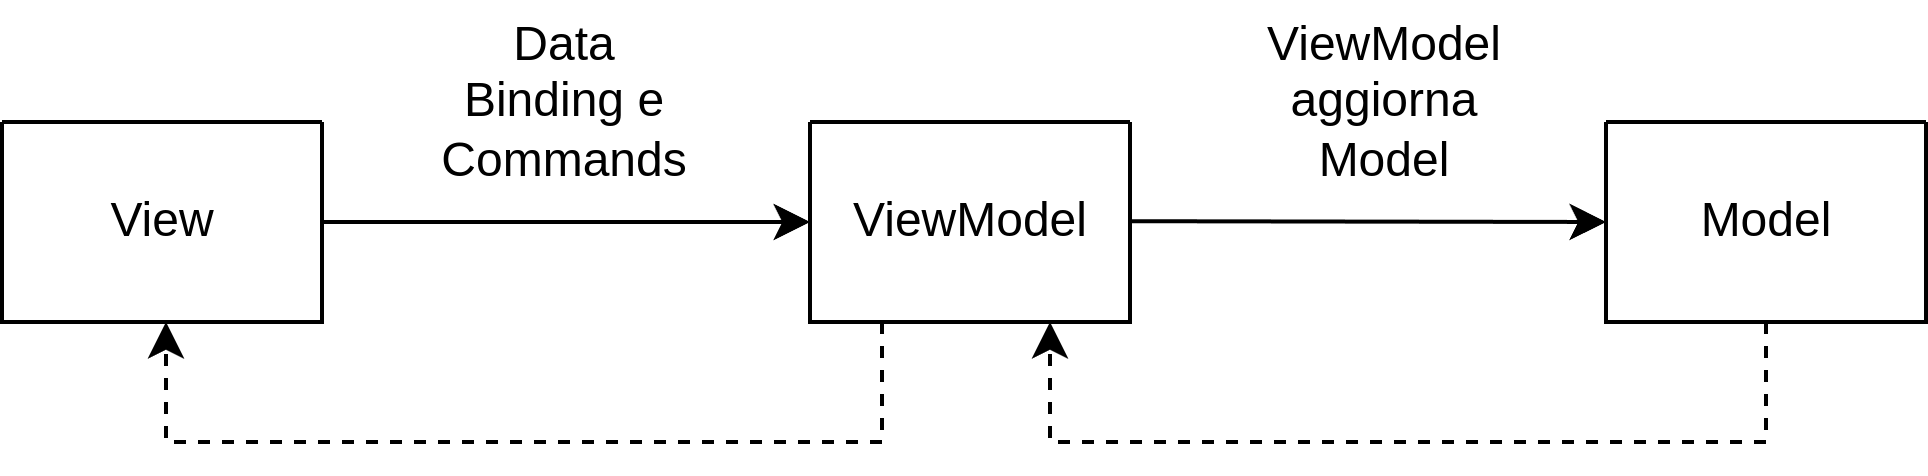
\includegraphics[width=.9\columnwidth]{images/MVVM.png} 
    \caption{Struttura del \emph{Model-View-ViewModel}}
\end{figure}

I tre \emph{namespace} principali del frontend sono quindi:
\begin{enumerate}
    \item \verb+MoviExpense.Models+;
    \item \verb+MoviExpense.Views+;
    \item \verb+MoviExpense.ViewModels+.
\end{enumerate}

\subsection{MoviExpense.Models}
\label{cap:model}

Questo \emph{namespace} contiene le classi che rappresentano gli oggetti di dominio dell'applicazione. Le quattro classi principali sono \verb+User+, \verb+Utente+, \verb+Spesa+ e \verb+NotaSpese+.

\begin{namespacedesc}
    \classdesc{User}{è la classe utilizzata per l'autenticazione nel sistema. Contiene Username e Password presi dal form di login, un booleano che conferma o meno il salvataggio delle credenziali e il token di autenticazione, inizialmente lasciato vuoto e assegnato quando l'identità viene confermata.}
    \classdesc{Utente}{rappresenta l'utente autenticato. È dotata di Id, username, codice utente, email, descrizione e il valore TariKm, che indica la tariffa di rimborso chilometrico per spese di carburante.}
    \classdesc{Spesa}{rappresenta l'oggetto principale dell'applicazione, ovvero la spesa che viene registrata. Contiene una serie di Id oltre al proprio, che vanno a identificare:
    \begin{itemize}
        \item la nota in cui è inserita;
        \item l'utente che registra la spesa;
        \item la causale;
        \item il tipo di pagamento;
        \item il fornitore presso cui è stata effettuata la spesa;
        \item la valuta con cui è stata effettuata.
    \end{itemize}
    \noindent Oltre a questi dati sono presenti le informazioni proprie della spesa, come l'importo, la data, il numero e la data della fattura, se emessa. Sono presenti poi alcuni flag booleani che indicano se è presente una fattura, se la spesa è stata selezionata per essere inserita in una nota, se è rimborsabile e se è stata effettuata entro il comune di sede dell'azienda. Infine è presente un attributo che indica lo stato della spesa, il quale verrà spiegato nel dettaglio all'interno del prossimo capitolo.
    }
    \classdesc{NotaSpese}{modella una nota spese, ovvero un insieme di spese da inviare all'amministrazione dell'azienda. Ogni nota è identificata da un Id, ed è dotata di:
    \begin{itemize}
        \item descrizione (ad esempio "Spese rimborsabili luglio 2024");
        \item data in cui viene effettuata;
        \item un check che segnali se è una nota rimborsabile o meno;
        \item Id dell'utente che registra la nota.
    \end{itemize}
    \noindent Sono presenti anche un flag IsEditable che indica se la nota è modificabile e un intero che rappresenta lo stato della nota. Come per le spese, anche lo stato delle note sarà illustrato nel dettaglio nel prossimo capitolo.
    }
\end{namespacedesc}

\noindent All'interno del \emph{namespace} si trovano altre classi minori, che rappresentano attributi per le spese, come la causale, il tipo di pagamento o l'allegato, oppure altre entità dell'applicazione, ad esempio i totali delle spese divisi per determinate categorie.

\subsection{MoviExpense.Views}

Ogni classe di questo \emph{namespace} rappresenta una pagina dell'applicazione. Le pagine sono scritte utilizzando XAML, linguaggio prediletto di Xamarin.Forms, e per ogni file \verb+.xaml+ che definisce la struttura e l'aspetto della pagina, è presente un file \verb+.xaml.cs+ che inizializza tutte le componenti, carica le informazioni statiche nella pagina (ad esempio stringhe) e definisce i \emph{binding} con la ViewModel. Il nome di ogni file di questo \emph{namespace}, e di conseguenza ogni classe, termina con la parola "Page".

\begin{namespacedesc}
    \classdesc{LoginPage}{presenta il logo dell'applicazione e due \emph{entry} per inserire username e password.}
    \classdesc{HomePage}{contiene un breve testo di benvenuto e due pulsanti, uno per accedere alla pagina della spese, l'altro per accedere alla pagina delle note. In basso è presente una label che mostra il numero di versione dell'app.}
    \classdesc{SpesePage}{mostra la lista della spese associate all'utente presenti nel database. Queste sono filtrabili in base allo stato della spesa oppure possono essere mostrate tutte insieme. Da qui è possibile eliminare una spesa che sia ancora modificabile, visualizzarne i dettagli, creare una nuova spesa oppure accedere alla pagine di visualizzazione dei totali delle spese (TotaliSpesePage).}
    \classdesc{ViewEditSpesaPage}{questa pagina presenta una sorta di form per la creazione, modifica o solamente visualizzazione di una spesa. Da questa pagina è possibile raggiungere le pagine di selezione (SelCauPage, SelValutaPage, \dots), nelle quali si possono selezionare alcuni campi della spesa, come la causale, la valuta, il tipo di pagamento e il fornitore.}
    \classdesc{NotePage}{offre le stesse funzionalità di SpesePage ma è basata sulle note spese associate all'utente e presenti nel database. Non è possibile, però, visualizzare i totali.}
    \classdesc{ViewEditNotaPage}{permette di compilare un form per la creazione di una nota spesa. Da qui si può accedere alla pagina AddSpesePage, utile ad inserire le spese desiderate nella nota, ed è possibile accedere alla visualizzazione dei totali di tali spese.}
\end{namespacedesc}

\subsection{MoviExpense.ViewModels}

Per ogni classe della View e del Model è presente una classe di ViewModel, in particolare queste sono distinte dal nome: le classi associate alla View hanno lo stesso nome che hanno nella View ma sostituiscono la parola "Page" finale con "Manager" (ad esempio a \verb+ViewEditSpesaPage+ corrisponde \verb+ViewEditSpesaManager+), mentre quelle associate al Model hanno lo stesso nome che hanno nel Model ma preceduto da "Vm" (alla classe \verb+Spesa+ corrisponde la classe \verb+VmSpesa+).\\
Le classi "Vm" sono utilizzate dalla ViewModel per comunicare con il Model. Hanno come attributo un oggetto del Model di cui effettuano il \textit{property wrap}, ovvero gestiscono i meccanismi di modifica e accesso alle proprietà della classe del Model. Questo permette di avere una migliore sincronizzazione dei dati tra Model e View, anche grazie al meccanismo di notifica presente in queste classi. Tutte le classi della ViewModel implementano l'interfaccia \verb+INotifyPropertyChanged+, a cui appartiene il metodo \verb+OnPropertyChanged+ che permette di notificare alla View i cambiamenti nei dati del Model, così che possano essere effettuate le modifiche necessarie all'interfaccia grafica. Di seguito è riportato un esempio di \textit{property wrapping}:
\begin{minted}[linenos, breaklines, frame=lines, framesep=5mm]{csharp}
    public int IdSpesa
    {
        get => Spesa.IdSpesa;
        set
        {
            Spesa.IdSpesa = value;
            OnPropertyChanged(nameof(IdSpesa));
        }
    }
\end{minted}

\noindent Le classi "Manager", invece, effettuano il \emph{binding} con la View e si occupano di:
\begin{itemize}
    \item comunicare con le API;
    \item gestire i dati non statici, ovvero di tutti i dati presi da database, e che possono quindi subire modifiche durante l'utilizzo dell'app;
    \item gestire i comandi inviati dalla View. Ad esempio quando si clicca l'icona per eliminare una spesa, viene chiamato un metodo di una classe "Manager" della ViewModel.
\end{itemize}

\vspace{1.5cm}

\noindent Oltre ai tre \emph{namespace} appena descritti, ne sono presenti altri di supporto. Tra questi i principali sono: MoviExpense.Converters che contiene dei convertitori utili ad esempio ad assegnare proprietà booleane legate a valori non booleani, e MoviExpense.Resources che contiene tutte le stringhe dell'applicazione. L'immagine seguente riporta come viene visualizzato il file Resources principale su Visual Studio.

\begin{figure}[H]
    \centering
    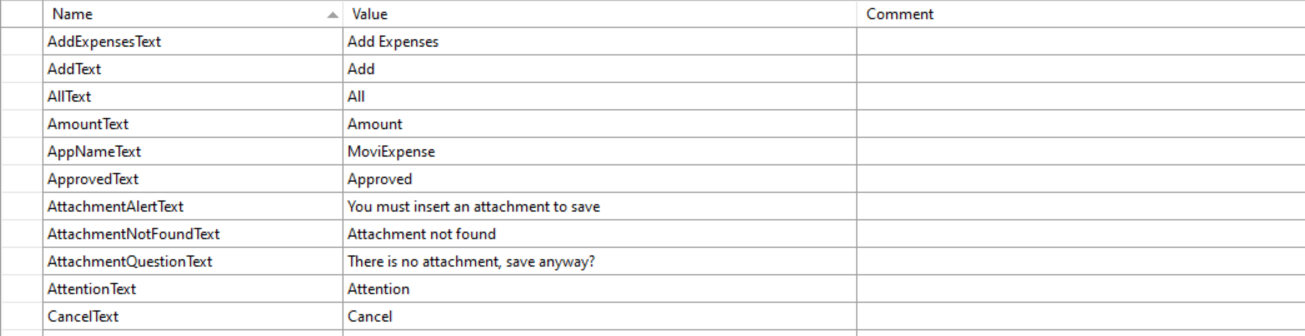
\includegraphics[width=\columnwidth]{images/resources.png}
    \caption{File Resources.resx aperto in Visual Studio}
\end{figure}



\section{Backend}

\subsection{API}

Entrambe le \glox{API} si basano su un'architettura layered a tre livelli:
\begin{enumerate}
    \item \textbf{Presentation layer}: livello di accesso a cui arrivano le chiamate;
    \item \textbf{Business layer}: si occupa di elaborare le chiamate ed indirizzarle al database;
    \item \textbf{Data Access layer}: livello che modella i dati del database in oggetti di dominio.
\end{enumerate}

\noindent Il funzionamento generale delle \glox{API} è il seguente:
\begin{enumerate}
    \item viene effettuata una chiamata http dall'esterno (dal frontend o da un'altra API);
    \item la chiamata viene intercettata dal Controller specifico che utilizza un oggetto Service per chiamare il metodo corrispondente alla chiamata http ricevuta;
    \item il Service "inoltra" la chiamata a una classe specifica del business layer;
    \item nel business layer si utilizza un oggetto ExpContext per accedere al database;
    \item i dati prelevati o inseriti nel database sono modellati con un oggetto del data accesso layer.
\end{enumerate}

\noindent Di seguito è riportato il funzionamento delle \glox{API} in modo \emph{top-down} attraverso i \emph{namespace} in cui avvengono le chiamate. Dato che entrambe le \glox{API} funzionano in modo analogo, nei nomi dei \emph{namespace} sarà presente \verb+[NomeAPI]+, che potrà essere quindi "Gateway" o "DataProvider".

\subsubsection{MoviExpense.Api.[NomeApi].Controllers}

È presente una classe Controller per ogni classe del modello (SpesaController, CausaleController, \dots). Questo \emph{namespace} rappresenta il livello di accesso alle API, è il \emph{namespace} che accoglie le chiamate http emesse dall'esterno.\\
Ogni classe Controller ha un attributo della classe ad esso associata nel \hyperref[cap:services]{\emph{namespace} seguente} e un metodo per ogni chiamata che possono ricevere. Questi metodi sono identificati tramite attributi di routing, ad esempio la Get generale nella classe SpesaController ha il seguente attributo di routing

\begin{minted}[linenos, breaklines, frame=lines, framesep=5mm]{csharp}
    [HttpGet] //Attributo di routing
    public IActionResult Get(int filterType, bool rimborsabile) {...}
\end{minted}

\noindent Anche la classe stessa è identificata da diversi attributi, in particolare:
\begin{itemize}
    \item \verb+[Authorize]+: indica che è necessario essere autenticati per accedere alle funzionalità dell'API;
    \item \verb+[Route("api/[controller]")]+: specifica parte dell'url dell'API;
    \item \verb+[ApiController]+: consente di abilitare gli attributi di routing, le risposte automatiche per i codici di errore 400 e il binding con attributi come \verb+[FromBody]+, \verb+[FromForm]+, \dots
\end{itemize}
All'interno di ogni metodo costruiscono un oggetto di tipo Param, costituito da username dell'utente e codice dell'azienda associata, e chiamano il metodo del Service corrispondente alla chiamata ricevuta. Nel caso della Get inserito prima viene
chiamato \verb+_service.GetAll(...)+, dove \verb+_service+ è di tipo \verb+ISpesaService+.

\subsubsection{MoviExpense.Api.[NomeApi].Services}
\label{cap:services}

È presente un'interfaccia e una classe concreta Service per ogni Controller (ISpesaService, SpesaService, ICausaleService, CausaleService, \dots). Ogni classe concreta ha come attributo un oggetto del \emph{namespace} \verb+MoviExpense.Api.[NomeApi].BL+, tramite cui chiama un metodo del business layer corrispondente alla chiamata http ricevuta.\\
Continuando l'esempio iniziato precedentemente, ci sarà un oggetto \verb+SpesaBL bl+ che nel metodo \verb+public List<SpesaEstesa> GetAll(...)+ chiamato dal Controller effettuerà la chiamata \verb+bl.GetAll(...)+.

\subsubsection{MoviExpense.Api.[NomeApi].BL e MoviExpense.Api.[NomeApi].DAL}

DAL ha il compito di modellare i dati del database in oggetti di dominio, di conseguenza avrà una classe per ogni tipo di oggetto (Spesa, Causale, \dots). Questi oggetti sono utilizzati nelle classi BL.\\
Nelle classi BL viene ricavata la stringa di connessione al database aziendale tramite il database Sys, e utilizzati degli oggetti ExpContext per effettuare la connessione ed eseguire le query necessarie a soddisfare la chiamata http ricevuta.

\subsubsection{Gateway}

Il funzionamento delle \glox{API} Gateway corrisponde a quello delle DataProvider solamente per effettuare Get sui dati dell'utente autenticato e per effettuare l'autenticazione (in questo caso c'è solamente una chiamata ulteriore). In tutti gli altri casi, il loro funzionamento è uguale solamente fino alla sezione riguardante i Services. Quando la chiamata arriva a una classe del \emph{namespace} MoviExpense.Api.Gateway.Services, infatti, non viene inoltrata al BL ma viene ricavato da CommonDb l'url delle \glox{API} data provider corrispondenti all'azienda dell'utente e la chiamata viene inoltrata a queste.

\paragraph{Autenticazione} Come detto in precedenza, le \glox{API} gateway in caso di autenticazione funzionano allo stesso modo delle data provider, con una sola aggiunta. Quando si arriva al BL, dopo aver effettuato la query su CommonDb per verificare che l'utente esista e le credenziali siano corrette (utilizzando una classe del DAL), viene chiamato un metodo del \emph{namespace} MoviExpense.Api.Gateway.Authentication, che contiene la classe Engine. Questa classe permette la gestione dell'autenticazione JWT ed è responsabile della generazione del token di autenticazione per l'utente.


\subsection{Database}

Come si può vedere nella \figref{fig:microservizi}, nel sistema dell'applicazione sono presenti tre database: CommonDb, SysDb e un database aziendale.

\subsubsection{CommonDb}

Viene utilizzato per:
\begin{itemize}
    \item autenticazione (tabella Utente);
    \item recupero delle informazioni dell'utente (tabella Utente);
    \item recuperare il numero di versione dell'applicazione (tabella AppInfo);
    \item recupero dell'url delle \glox{API} data provider (tabelle UtenteAzienda e Azienda).
\end{itemize}

\subsubsection{SysDb}

Contiene una sola tabella chiamata Azienda, che viene utilizzata per ricavare i parametri utili a costruire la stringa di connessione per il database aziendale.

\subsubsection{Database aziendale}

\begin{figure}[H]
    \centering
    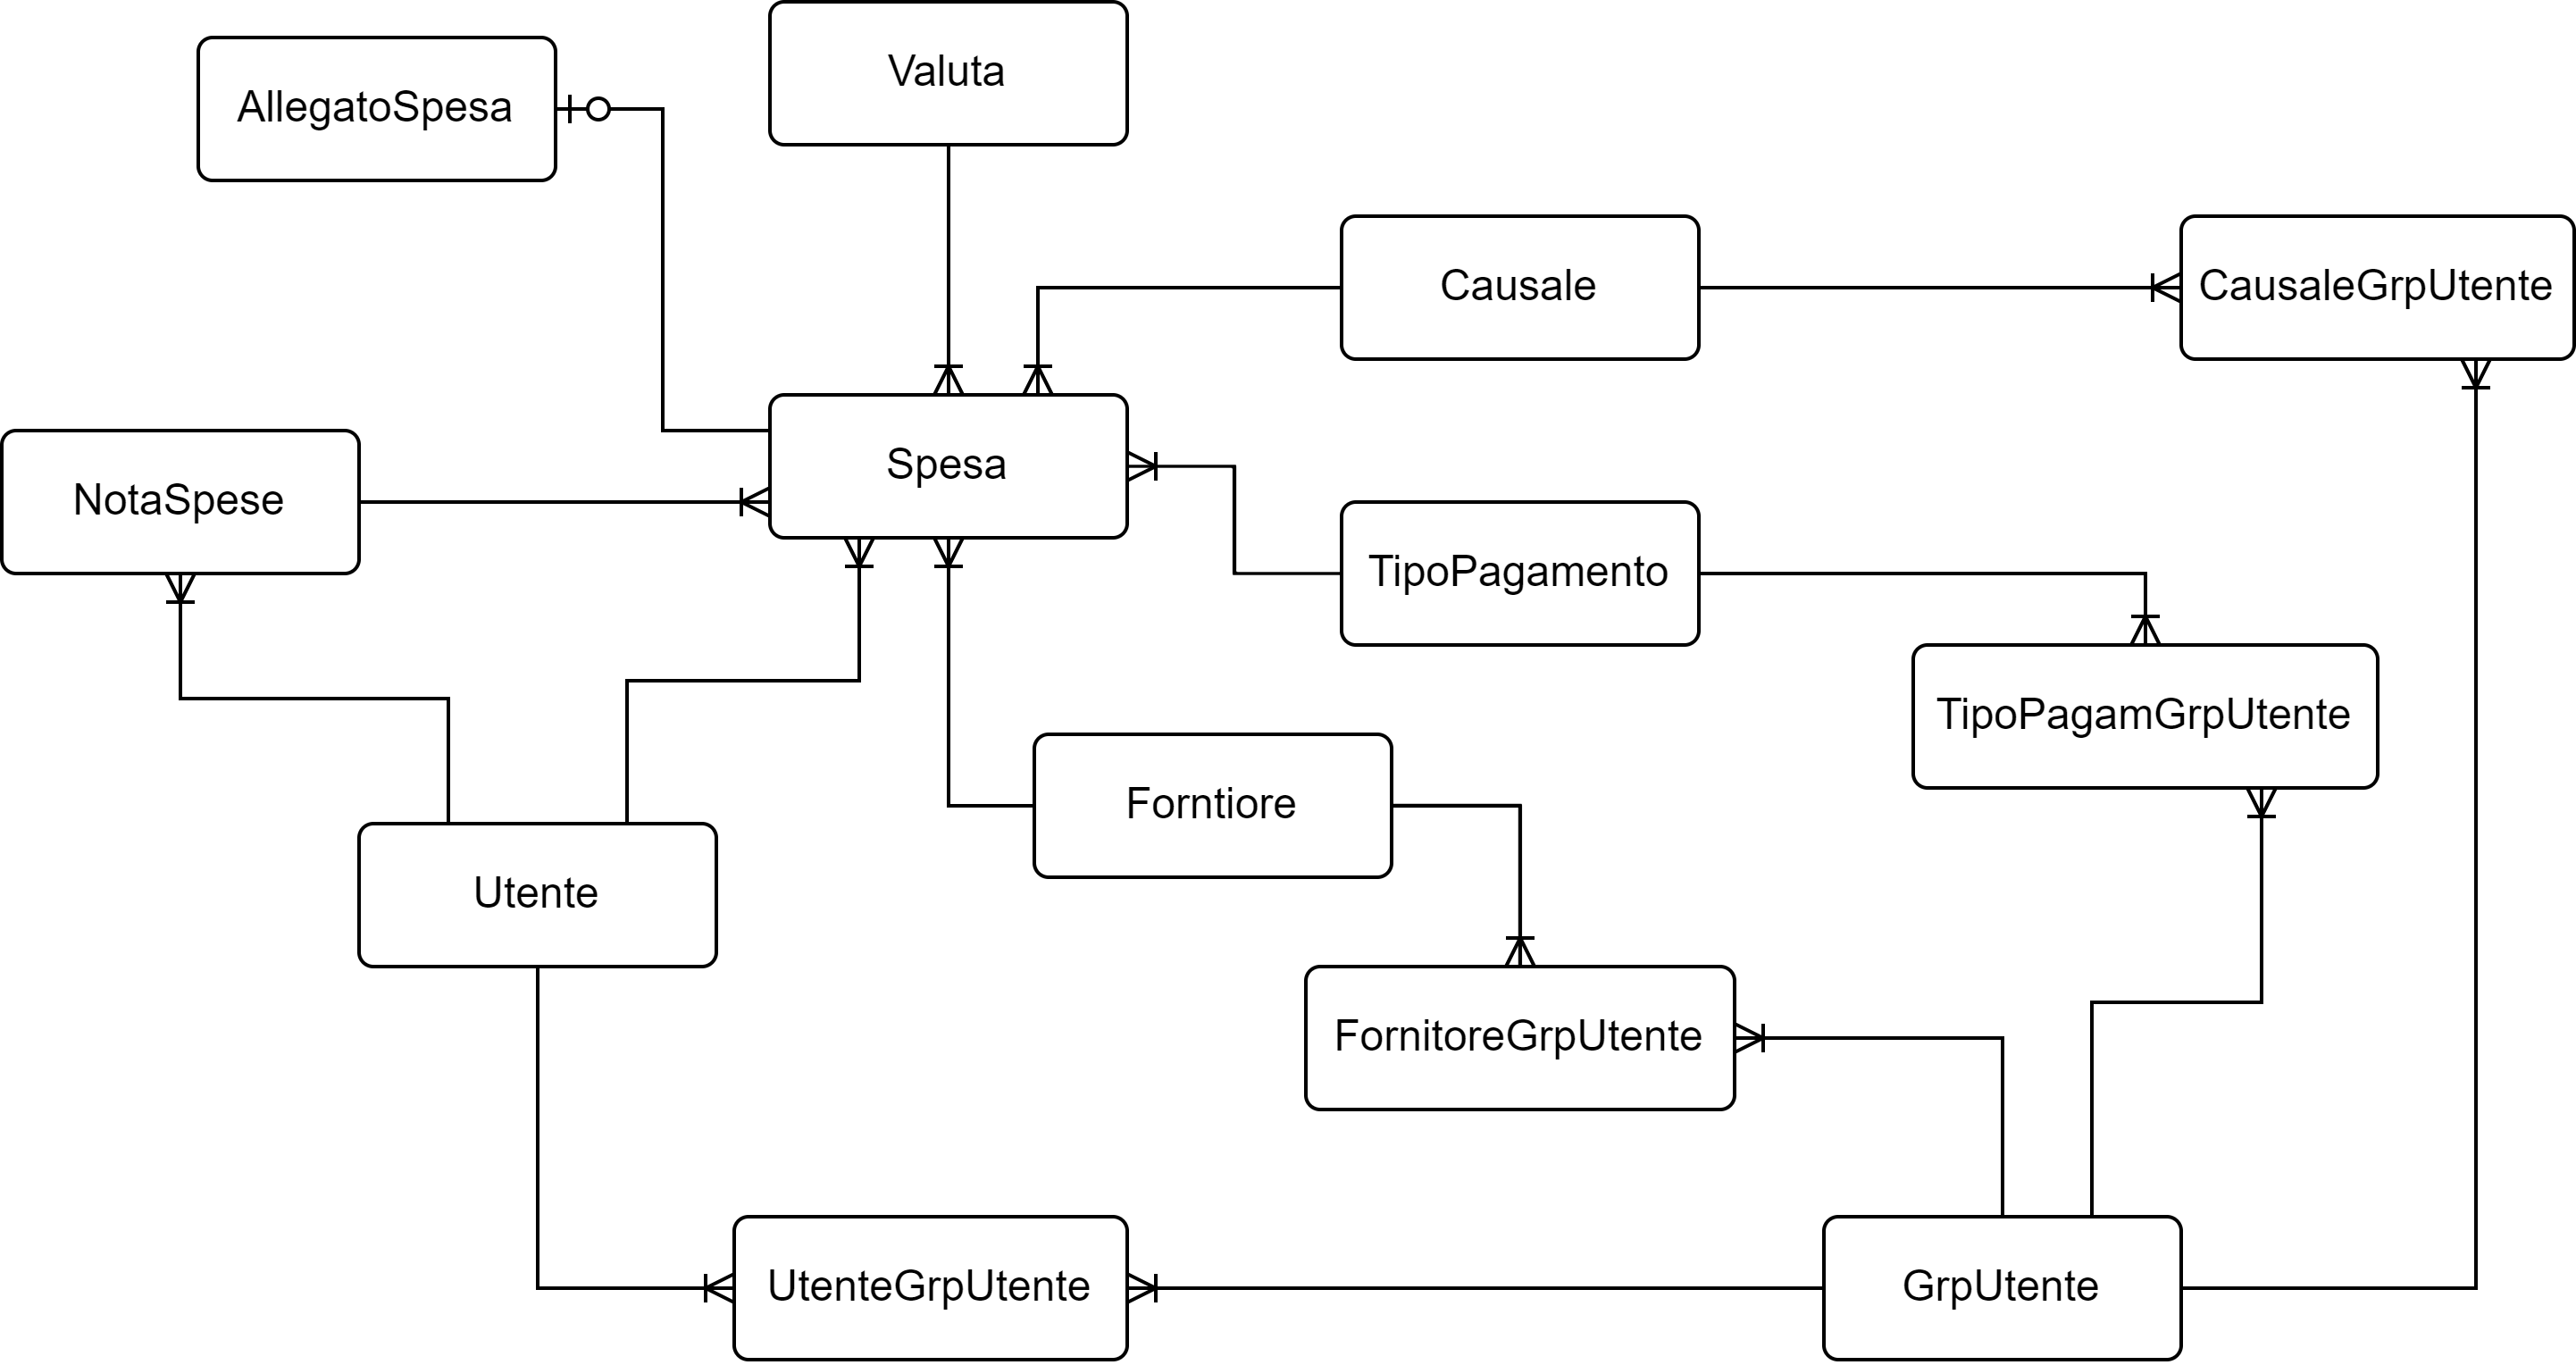
\includegraphics[width=\columnwidth]{images/ER moviEXPENSE.png}
    \caption{Schema ER database aziendale}
\end{figure}
